% !TEX encoding = UTF-8 Unicode
%!TEX root = thesis.tex
% !TEX spellcheck = en-US
%%=========================================
\chapter{Implementation and Simulation of Sensors}
Using electronic nautical charts (ENC), information about other simulated agents and 3D models of installations in sea it is possible to generate realistic sensor data for HIL simulations. This section contains an overview of the implementation of important sensors used on Odin and a brief discussion about how sensor data can be simulated. The Inertial Measurement Unit (IMU) is documented in (\textbf{Evens rapport, trenger referanse?}).

\section{Sensors for Environmental Analysis Implemented on Odin}
\label{SensorOverview}
In section \ref{SensorOverview} a brief overview of the sensors on Odin used for situational awareness above the surface are presented. The overall layout of sensors and system architecture are visualized in Figure \ref{fig:systemArchitecture}.

\begin{figure}[H]
	\begin{center}
		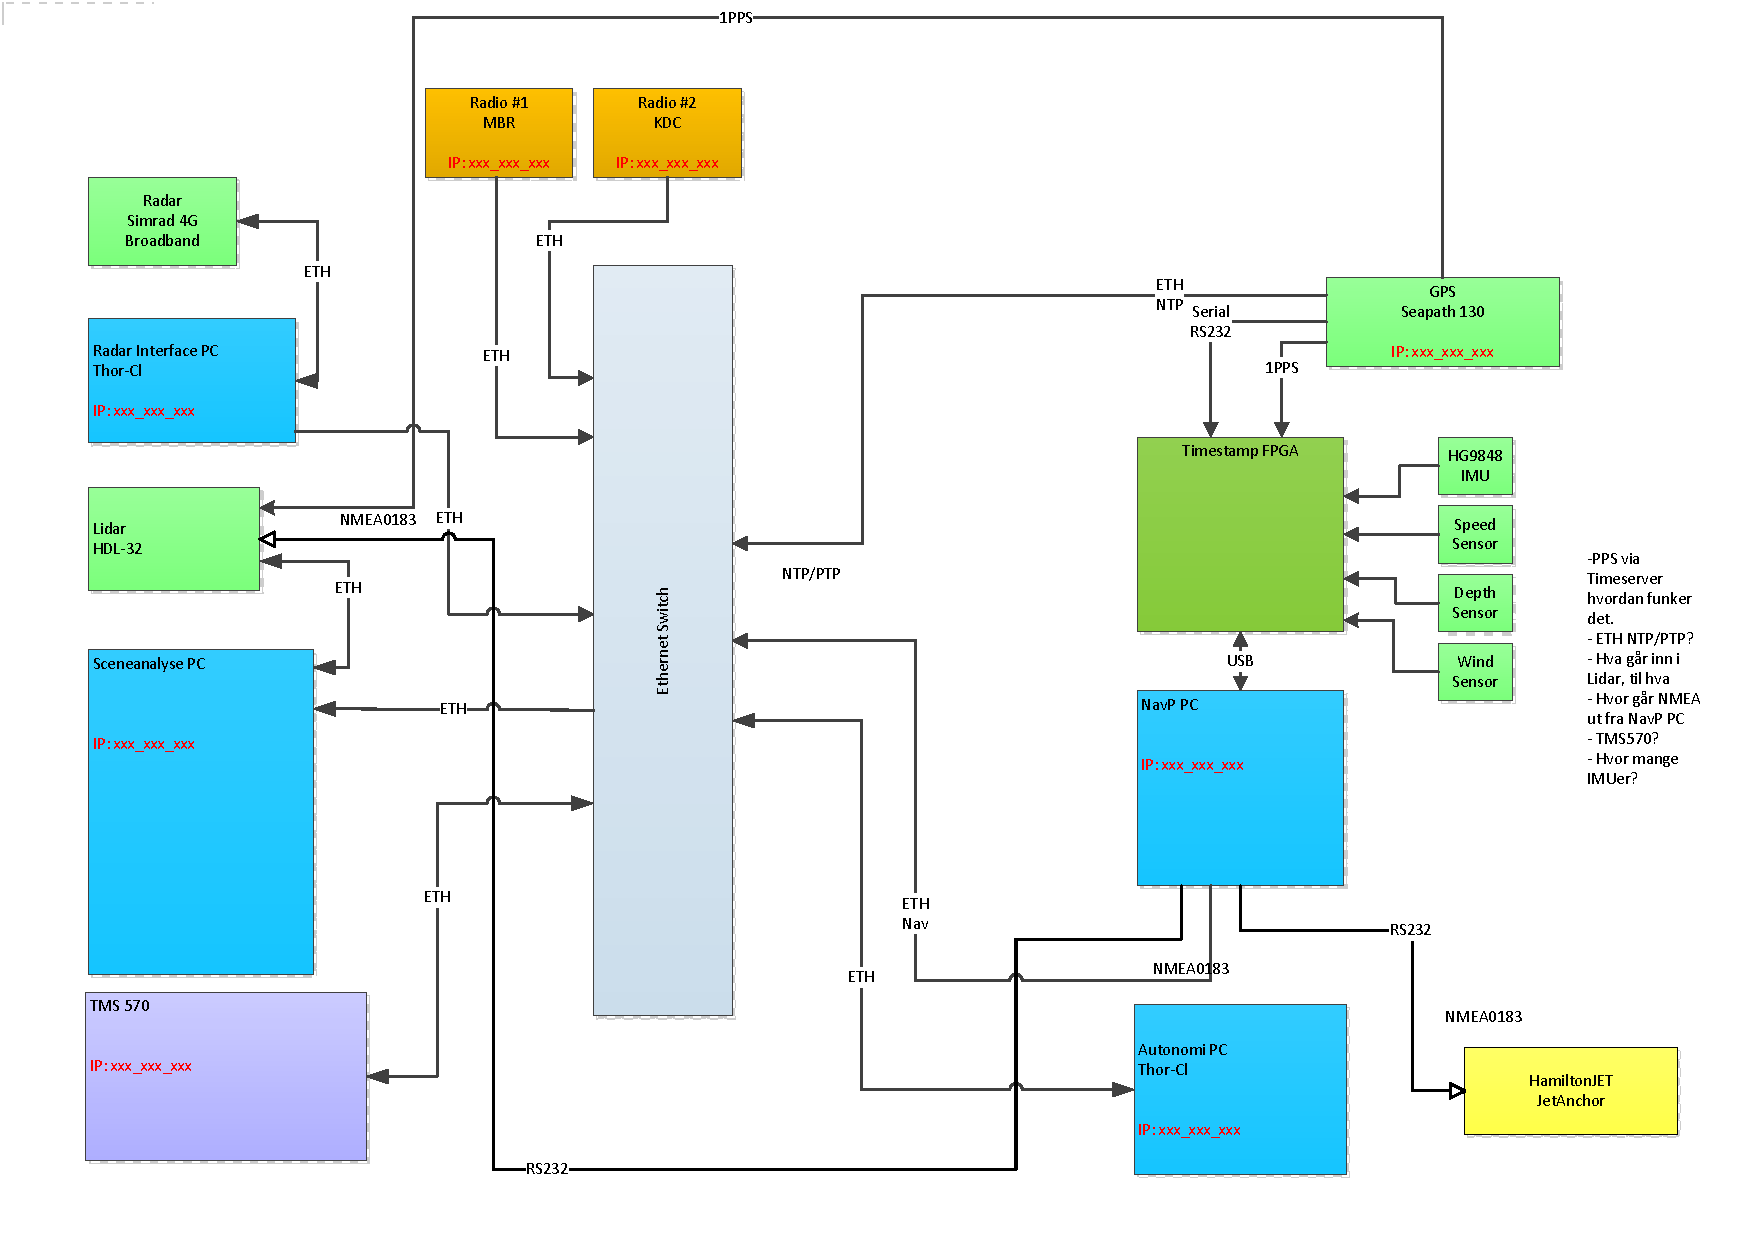
\includegraphics[width = 1\linewidth]{fig/SystemarkitekturOdin.pdf}
		\caption{\textit{Visualization of system architecture and network layout on Odin, including sensors and processing units.} \textbf{A better figure should be made when the final layout is determined!}}
		\label{fig:systemArchitecture}
	\end{center}
\end{figure}

\subsection{Seapath 134 GPS}
The GPS used on Odin is the Seapath 134 developed by Kongsberg Seatex. Combining GNSS signals and IMU data the Seapath 134 gives highly accurate heading, position, heave, roll and pitch measurements (\cite{SeapathManual}). Data is transmitted via standard NMEA 0183 protocol (\cite{NMEAmanual}) over a serial RS232 cable for interpretation by the control system. \textbf{Short introduction and small example of NMEA protocol should come here.}

\begin{figure}[H]
	\begin{center}
		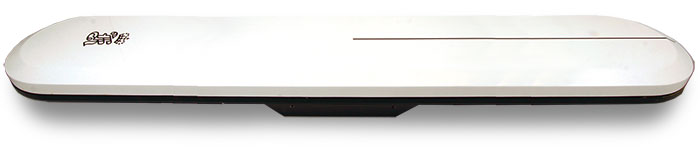
\includegraphics[width = 0.7\linewidth]{fig/Seapath130.jpg}
		\caption{\textit{The Seapath 134 developed by Kongsberg Seatex is used on Odin for position, heading and attitude measurements.}}
		\label{fig:seapath130}
	\end{center}
\end{figure}

\subsection{Radar}
\begin{wrapfigure}[7]{r}{0.3\textwidth}
	\vspace{-30pt}
	\begin{center}
		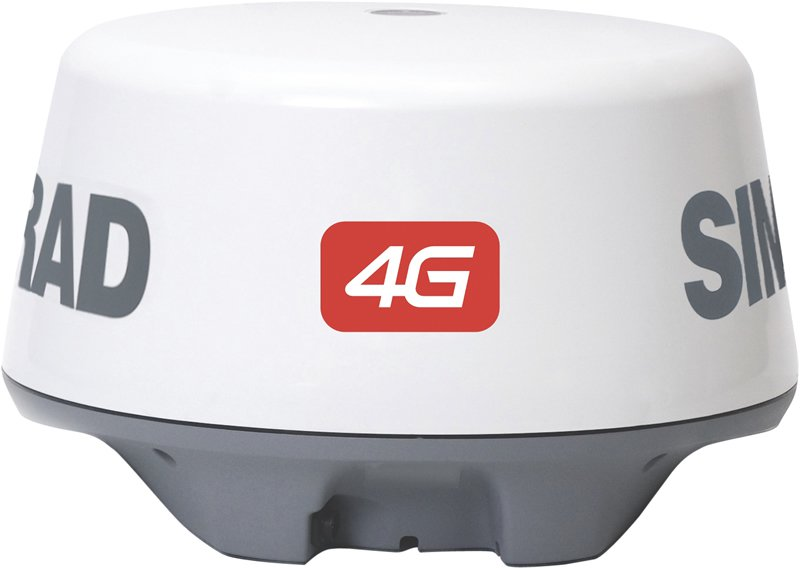
\includegraphics[width= 0.9\linewidth]{fig/navico4G}
		\vspace{-10pt}
		\caption{\it{Simrad Broadband 4G radar used on Odin.}}
		\label{fig:navico4G}
	\end{center}	
\end{wrapfigure}
The radar used on Odin is a Simrad Broadband 4G with range from 200 feet to 32 nautical miles and 48 RPM sweep  rate (\cite{simradBrochure}). The radar communicates directly with the \textit{Radar Interface PC} as seen in Figure \ref{fig:systemArchitecture}. Automatic Radar Plotting Aid (ARPA) (\cite{ARPAmanual}) is used for target tracking and analysis in the radar interface. It is assumed that the radar interface including the ARPA functionality is well tested and that the output from \textit{Radar Interface PC} is predictable and well documented, possibly following some NMEA like protocol. At the current time the details of the transaction of this information is not yet decided. Processed target and surroundings data is transmitted via Ethernet and is assumed to at least include information about target position, heading and speed. Other possibly available data might be time and point of collision, radar cross section (or other target size information) and current noise conditions.\\


\newpage
\subsection{Velodyne LiDAR HDL-32E}
\begin{wrapfigure}[14]{l}{0.3\textwidth}
	\vspace{-30pt}
	\begin{center}
		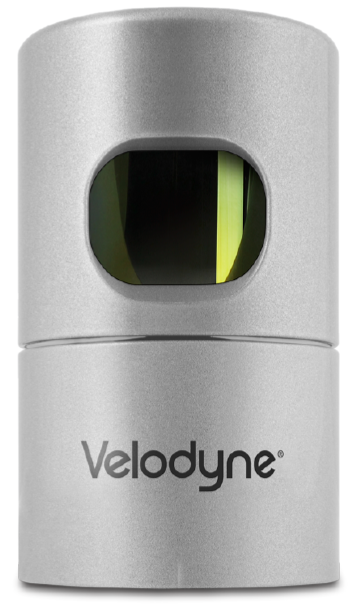
\includegraphics[width= 0.9\linewidth]{fig/VelodyneHDL32Ecase}
		\vspace{-20pt}
		\caption{\it{Velodyne LiDAR HDL-32E used on Odin for above-the-surface 3D analysis.}}
		\label{fig:velodyneCasing}
	\end{center}
	
\end{wrapfigure}
For analysis of the nearby environment above the surface a LiDAR is used to create a 3D point cloud. The model used on Odin is a Velodyne HDL-32E as seen in Figure \ref{fig:velodyneCasing}. A LiDAR can measure the distance to points around the sensor by firing a laser and measure the time it takes for the light to return. The distance is then saved along with the horizontal and vertical angle of the laser, so that the positions of the measured points can be used to generate a 3D model of the nearby environment. Velodyne HDL-32E generates 700,000 points per second with $\pm2$cm accuracy at 80m-100m range. The LiDAR spins around the vertical axis to achieve a $360\degree$ horizontal field of view (FOV), and a combination of 32 lasers stacked vertically yields a $40\degree$ vertical FOV ($+10\degree$ to $-30\degree$). An external GPS should be connected to the LiDAR for time pulse synchronization.

Uncalibrated point cloud data packets are transmitted from the LiDAR over a standard Ethernet cable using UDP. The packet format is well documented in the user manual so that they should be easy to decompose by a custom made point cloud processing unit. A calibration table must be used for vertical correction for each laser. This table is included on a CD delivered with the HDL-32E.

The LiDAR sweeps are processed by \textit{Sceneanalys PC} as seen in Figure \ref{fig:systemArchitecture}. The data is stored in a ROS structure called \texttt{grid\_map} and sent to the motion planning module in \textit{Autonomi PC} (Figure \ref{fig:systemArchitecture}). Detected objects are planned to be put in ROS messages containing information about relative position, speed, heading, latitude/longitide and detection probability.


\section{Simulation of Sensor Data from Virtual Environment}
The feasibility of simulating realistic sensor data from a virtual environment will be discussed in this section, as well as complexity and benefits regarding simulation of raw versus preprocessed sensor data. Information, hardware and software needed to generate data from each sensor will also be discussed.

\subsection{Simulating Data from GPS}
As the data output of the Seapath 134 follows the well documented NMEA0183 protocol it should be feasible to generate these data based on knowledge of position, speed, heading and attitude. This information should be a result of simulating the boats motion in the virtual environment and is thereby easily accessible.
\remark{ In the system architecture (Figure \ref{fig:systemArchitecture}) of Odin the GPS is used for time synchronization of the entire system. It is assumed that the HIL setup is synchronized in time using either NTP or PTP network timing. A real or simulated GPS time synchronization signal is therefore not considered necessary in the scope of this project. 

\subsection{Simulating Data from Radar}
Assuming predictable and well documented data output from \textit{Radar Interface PC} (Figure \ref{fig:systemArchitecture}) it should be feasible to simulate output from this subsystem given information about simulated targets around Odin. Simulating raw data from the radar, i.e simulating the exact radio signal reflected from the target, is considered too complex to stay within the scope of this project. This is because it requires too detailed information about everything from the target shape, weather conditions and the specific radar in use as well as a deep understanding of radar technology. It is thereby determined that only preprocessed data from the \textit{Radar Interface PC} will be simulated. To simulate realistic output the following points should be considered:

\begin{itemize}
	\item Radar blind zones minimum detection range.
	\item Radar range being dependent on weather conditions. 
	\item Target detection dependent on the shape and orientation of target.
	\item During precipitation clutter a target may or may not be detected. A solution could be to use a randomize function to determine if a target should be detected or not. In that case, reproducibility of simulation might be more difficult.
	\item Accuracy of the implemented radar and how to model errors resulting from inaccuracy. \cite{ARPAmanual} gives great details about possible errors.
\end{itemize}

\subsection{Simulating Data from LiDAR}
The protocol of the data transfer from Velodyne HDL-32E is well documented. Given a 3D model of the surrounding environment with easy access to angle and distance calculations it should be feasible to generate a realistic point cloud. The point cloud can be represented as data packets using the HDL-32E protocol and sent over Ethernet to the interface between HIL simulator and the control system. This way it would be possible to simulate raw sensor readings from the HDL-32E. This is assumed to be beneficial to the developers of the simulated vehicle as a larger chain of HW/SW can be tested in the simulated environment. A challenge with this approach is to simulate realistic sensor readings during rainy conditions and other environmental disturbances. A solution could be to use randomized noise added to the simulated measurements. A deterministic randomize function should be used to ensure reproducibility of the simulations. 3D modeling of the surrounding environment might also be computationally challenging. More research should be done to investigate the feasibility of this.\\ 
\\
As shown in Figure \ref{fig:systemArchitecture}, the data from the LiDAR is processed by the \textit{Sceneanalyse PC}. If this module is well tested, or the 3D processing of the surrounding environment is too computationally heavy, it might be more convenient to simulate the output from this PC directly without going through the steps of generating a point cloud. \textbf{The output from \textit{Sceneanalyse PC} is what? Possibly strings with information about nearby targets? Would be easy to generate.}







